\documentclass[letterpaper,twocolumn]{article}

\usepackage[top=1in,bottom=1in,left=0.75in,right=0.75in]{geometry}
\usepackage{graphicx}
\usepackage{newtxtext}
\usepackage{newtxmath}
\usepackage[hyphens]{url}

% Better look for citations that include a section reference like \cite[\S 3]{foobar}.
\usepackage{cite}
\renewcommand{\citemid}{~}

% Load hyperref after other packages.
\usepackage[pdfa,hidelinks,pdfcreator={},pdfproducer={}]{hyperref}
\urlstyle{same}
\def\sectionautorefname{Section}
\def\subsectionautorefname{Section}

% Disable metadata for reproducible PDF.
% https://tex.stackexchange.com/a/313605
\usepackage{ifpdf}
\ifpdf
\pdfinfoomitdate=1
\pdftrailerid{}
\pdfsuppressptexinfo=-1
\fi

\hyphenation{Web-RTC}
\hyphenation{Java-Script}

\begin{document}

\date{}

\title{Snowflake, a peer-to-peer censorship circumvention system}

% ANON
\author{}

\maketitle

\begin{abstract}
\begin{itemize}
\item temporary proxies using WebRTC
\item central matching of proxies and clients
\item JavaScript browser add-on, or command-line proxies
\item deployed in Tor Browser
\item history of deployment and blocking attempts
\item observations for circumvention
\end{itemize}
\end{abstract}

% General references:
%   https://gitlab.torproject.org/tpo/anti-censorship/pluggable-transports/snowflake/-/wikis/Technical%20Overview
%   https://www.bamsoftware.com/papers/thesis/#chap:snowflake

\section{Introduction}
\label{sec:intro}

Put Snowflake in context

Spectrum of looks-like-nothing to looks-like-something

Spectrum of few, valuable proxies with careful distribution to
many, cheap proxies with less emphasis on secrecy

\section{Background}
\label{sec:background}

% serene, david

WebRTC

% hooman
- interacting suite of multiple protocols
- example applications
- importantly: built into browsers

flash proxy~\cite{Fifield2012a} (\url{https://bugs.torproject.org/legacy/trac/5578})
uProxy (\url{https://serene.cx/snowflake/})

Comparison with MassBrowser~\cite{Nasr2020a}
% https://github.com/net4people/bbs/issues/32

\section{How it works}

% serene, arlo

\begin{figure*}
\framebox[\textwidth]{\vbox to 2in{\vfil\centering TODO\vfil}}
\caption{
Architecture of Snowflake.
}
\label{fig:architecture}
\end{figure*}

\autoref{fig:architecture}

Centralized broker, manages associations between clients and proxies

% hooman
Centralized bridge
- (notionally centralized, though may be realized as multiple instances for performance reasons, see \autoref{sec:experience})

Decentralized proxies
- Clients do not touch the bridge directly, but only through a proxy
- No risk if the bridge itself is blocked
- Proxies can be blocked---even in the middle of an ongoing connection---and clients can adapt by switching to another proxy
- In practice, realized as browser add-ons or standalone executables

Many moving parts, managing complexity is a consideration

\subsection{Rendezvous}

% serene

Communication with broker has different anti-blocking requirements,
can be slower / more expensive

Contents of rendezvous messages
WebRTC signaling, ICE as part of WebRTC
requires bidirectional

Domain fronting remains an important element of circumvention systems,
though since the reaction by cloud providers
to the attempted blocking of Telegram in Russia in 2018,
% TODO: cite something
it is recognized that domain fronting should not be relied on exclusively.


domain fronting
AMP cache
others?
- DNS over encryption
- flash proxy could use email

long polling

\subsection{Temporary proxying}

% cecylia

Proxies are simple conduits, transferring a reliable stream between endpoints
End-to-end security between client and bridge, proxies untrusted

% david
Turbo Tunnel~\cite{Fifield2020a}
KCP/smux
- session layer independent of the circumvention channel, permits switching proxies on the fly
- the protocol layering generally

Web badge vs. browser add-on vs. standalone daemon
majority browser add-on, more effective at gaining popularity than web badge

% cecylia
NAT type matching (necessity of, and how it works)
probetest

\subsection{Protocol fingerprinting}

% kyle, david

\url{https://gitlab.torproject.org/tpo/anti-censorship/pluggable-transports/snowflake/-/wikis/Fingerprinting}

Fifield and Gil Epner~\cite{arxiv.1605.08805}

MacMillan et~al.~\cite{arxiv.2008.03254}

Snowflake leans heavily into the ``address blocking'' side of blocking
resistance, but the ``content blocking'' part is still important.

Fingerprintable features
- signaling
- STUN (choice of servers and contents of messages)
- DTLS
- WebRTC media channel vs. data channel

Historically overvalued in research (cf. \cite{Tschantz2016a})
Practicality is paramount; censors are hard to predict
But we can anticipate possible reactions

\section{Experience}
\label{sec:experience}

\begin{figure}
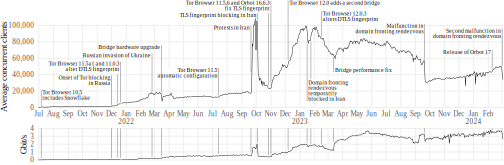
\includegraphics{figures/users-global/users-global}
\caption{
Estimated average number of simultaneous Snowflake users.
Loesing~\cite{tor-tr-2012-10-001}
describes how the number of users is estimated.
}
\label{fig:user-counts}
\end{figure}

% david
User count charts \autoref{fig:user-counts}
\url{https://bugs.torproject.org/tpo/network-health/metrics/website/40047\#note\_2796619}
- alpha release
- Turbo Tunnel
- stable release
- Russia blocking

% david
$X$ TB of user data transferred

% cecylia
Counts of web badge vs. browser add-on vs. standalone daemon
Cupcake
Relative ineffectiveness of web badge (i.e. the flash proxy model)
people love the add-on and the daily count of connections

scaling
- load balancing
- multi-bridge

Orbot? as both client and proxy?

\subsection{Development challenges}

% arlo, cecylia

Difficulty of using WebRTC outside a browser

Reproducible builds

Pion

\subsection{Blocking in Turkmenistan}

\begin{figure}
\framebox[\linewidth]{\vbox to 2in{\vfil\centering TODO\vfil}}
\caption{
Users in Turkmenistan and Russia,
around blocking events.
}
\label{fig:user-counts-tm-ru}
\end{figure}

\url{https://bugs.torproject.org/tpo/anti-censorship/censorship-analysis/40024}

\autoref{fig:user-counts-tm-ru}

Block of domain front
Unclear if AMP cache rendezvous was a sufficient workaround
Hard to get testers/volunteers

\subsection{Blocking in Russia}

% david

\autoref{fig:user-counts-tm-ru}

\url{https://bugs.torproject.org/tpo/community/support/40050}
\url{https://ntc.party/t/ooni-reports-of-tor-blocking-in-certain-isps-since-2021-12-01/1477}
% \url{https://blog.torproject.org/tor-censorship-in-russia/}

Snowflake blocked in Russia, along with all other Tor protocols,
in December 2021 \cite{ooni-2021-russia-blocks-tor}
In comparison to TM, easy to get testers
Managed to unblock it within 2 weeks

supported\_groups in Specific DTLS Server Hello Extension
Release to change fingerprint evaded blocking, has worked in Russia since
Had been anticipated by MacMillan et al.\cite[\S 3]{arxiv.2008.03254}
Though not necessarily the wrong call not to have prioritized a fix earlier
Importance during the invasion of Ukraine
- increased usage caused scaling difficulties
  \url{https://forum.torproject.net/t/tor-project-more-resources-required-for-snowflake-bridge/2353}

Second round of DTLS fingerprinting, this time targeting DTLS Client Hello?
\url{https://bugs.torproject.org/tpo/anti-censorship/censorship-analysis/40030#note_2803188}
\url{https://bugs.torproject.org/tpo/anti-censorship/pluggable-transports/snowflake/40140}
\url{https://ntc.party/t/a-new-snowflake-blocking-rule-offset-of-supported-groups-in-dtls-client-hello/2420}

\subsection{SQL injection attempts at broker}

% cecylia

\url{https://bugs.torproject.org/tpo/anti-censorship/pluggable-transports/snowflake/40089}
Actually tailored to the broker protocol, not a generic attack tool.

\subsection{Rate of proxy IP address churn}

% shelikhoo

Need a new experiment for this
\url{https://bugs.torproject.org/tpo/anti-censorship/pluggable-transports/snowflake/34075}

\subsection{Performance}
\label{sec:performance}

% cecylia

\section{Future work}

% shelikhoo

Distributed bridge architecture
\url{https://bugs.torproject.org/tpo/anti-censorship/pluggable-transports/snowflake/40129}

% ANON
% \section*{Availability}
%
% \url{https://snowflake.torproject.org/}

% ANON
% \section*{Acknowledgements}
%
% Griffin Boyce
% Chris Ball
% Tor Project
% Sukhbir Singh
% Ivan Markin (AMP cache)
% Pion (who at Pion?)
% ValdikSS (fingerprinting research during Russia blocking)
% Vern Paxson, CDT, OTF, anyone else Serene was involved with?
% Greenhost (eclips.is)
% Arthur Edelstein
% Linus Nordberg
% Mullvad (donated bridge hardware)
% volunteers running snowflake proxies
% anonymous donors

\bibliographystyle{plainurl}
\bibliography{snowflake}

\end{document}
